\appendix{h}
\chapter{Supplemental Material for Chapter 1}

%%%%%%%%%%%%%%%%%%%%%%%%%%%%%%%%%%%%%%%%%%%%%%%%%%%%%%%%%%%%%%%%%%%%%%%%%%%%%%%%
\section{Expression patterns of ZEE elements driving notochord expression}
%%%%%%%%%%%%%%%%%%%%%%%%%%%%%%%%%%%%%%%%%%%%%%%%%%%%%%%%%%%%%%%%%%%%%%%%%%%%%%%%

\subsection{Levels of expression for notochord-specific enhancers}
There are four notochord-specific enhancers (ZEE10, ZEE13, ZEE20, and ZEE27). The strongest of these is ZEE10, which is the only ZEE element in this group to contain a Bra site in addition to the Zic and ETS sites. We speculate that this additional Bra binding site could maintain and amplify the signal in a positive, feed-forward loop \cite{reeves2017}. ZEE13, ZEE20, and ZEE27 are all similar in their levels of expression, and we speculate that these enhancers have an organization of Zic and ETS sites that are permissive to notochord expression. 

\subsection{BraS and ZEE1 drive a6.5 expression}
BraS and ZEE1 have strong notochord expression, but also a6.5 expression. Zic and ETS are co-expressed in the a6.5 and notochord cell lineages \cite{matsumoto2007a}; thus, we think that the a6.5 expression seen in these constructs could be due to an organization of sites permissive to both neural and notochord expression. ZEE1 also has head endoderm expression, which could be due to the expression of FoxA and ETS in the endoderm or potentially other sites that we have yet to identify. The randomization of BraS rZEFB leads to a reduction in the number of embryos with a6.5 expression; this indicates that other sequences beyond the Zic, ETS, FoxA, and Bra sites contribute to the a6.5 expression. 

\subsection{ZEE35 and ZEE85 drive weak notochord expression with stronger ectopic expression}
ZEE35 and ZEE85 both drive weak notochord and stronger expression in other domains. ZEE85 drives strong expression in the b6.5 nerve cord; this expression could be due to ETS sites working in combination with other unidentified sites within the enhancer. ZEE35 drives strong expression in the endoderm, nerve cord, and a6.5 lineage. We speculate that this enhancer may contain an organization of sites that is optimal for binding of ETS in the endoderm and Zic and ETS in the a6.5 lineage. It is also possible that the organization of sites within these enhancers are not optimal for notochord expression, but more optimal for other domains of expression.

%%%%%%%%%%%%%%%%%%%%%%%%%%%%%%%%%%%%%%%%%%%%%%%%%%%%%%%%%%%%%%%%%%%%%%%%%%%%%%%%
\section{Supplementary Table Captions}
%%%%%%%%%%%%%%%%%%%%%%%%%%%%%%%%%%%%%%%%%%%%%%%%%%%%%%%%%%%%%%%%%%%%%%%%%%%%%%%%

The Supplemental Table can be found on the GitHub repository for this study labeled as \verb|SupplementaryTable.xlsx| at the following location: 

\noindent \href{https://github.com/mragsac/Diverse-Logics-Notochord-Study/}{\texttt{https://github.com/mragsac/Diverse-Logics-Notochord-Study/}}.

\par\noindent\dotfill

\subsubsection{Supplementary Table S1: All ZEE elements screened}
This table provides information about all ZEE elements: whether they were tested individually, their enhancer activity score, their genomic location, and their sequence.

\subsubsection{Supplementary Table S2: Scoring of ZEE elements individually tested}
This table provides scoring data for all three replicates of all ZEE elements chosen to be screened individually. Embryos were scored for no expression, expression and a6.5, b6.5, notochord, mesenchyme, and endoderm expression.

\subsubsection{Supplementary Table S3: Sequences of notochord elements}
This table provides the genomic location and sequence of notochord expressing ZEE elements.

\subsubsection{Supplementary Table S4: Scoring of manipulations on Lama and BraS enhancers}
This table provides scoring data for the manipulations of the Lama and BraS enhancers. Embryos were scored expression, no expression, notochord and a6.5 lineage expression.

\subsubsection{Supplementary Table S5: Oligonucleotides for Lama and BraS manipulations}
This table provides sequences for oligonucleotides used to mutagenize the Lama and BraS enhancers.

\subsubsection{Supplementary Table S6: Vertebrate enhancers referenced in this study}
This table provides genomic locations of vertebrate enhancers referenced in this study.

%%%%%%%%%%%%%%%%%%%%%%%%%%%%%%%%%%%%%%%%%%%%%%%%%%%%%%%%%%%%%%%%%%%%%%%%%%%%%%%%
\section{Supplementary Figures}
%%%%%%%%%%%%%%%%%%%%%%%%%%%%%%%%%%%%%%%%%%%%%%%%%%%%%%%%%%%%%%%%%%%%%%%%%%%%%%%%

\begin{figure}[h]
    \centering
    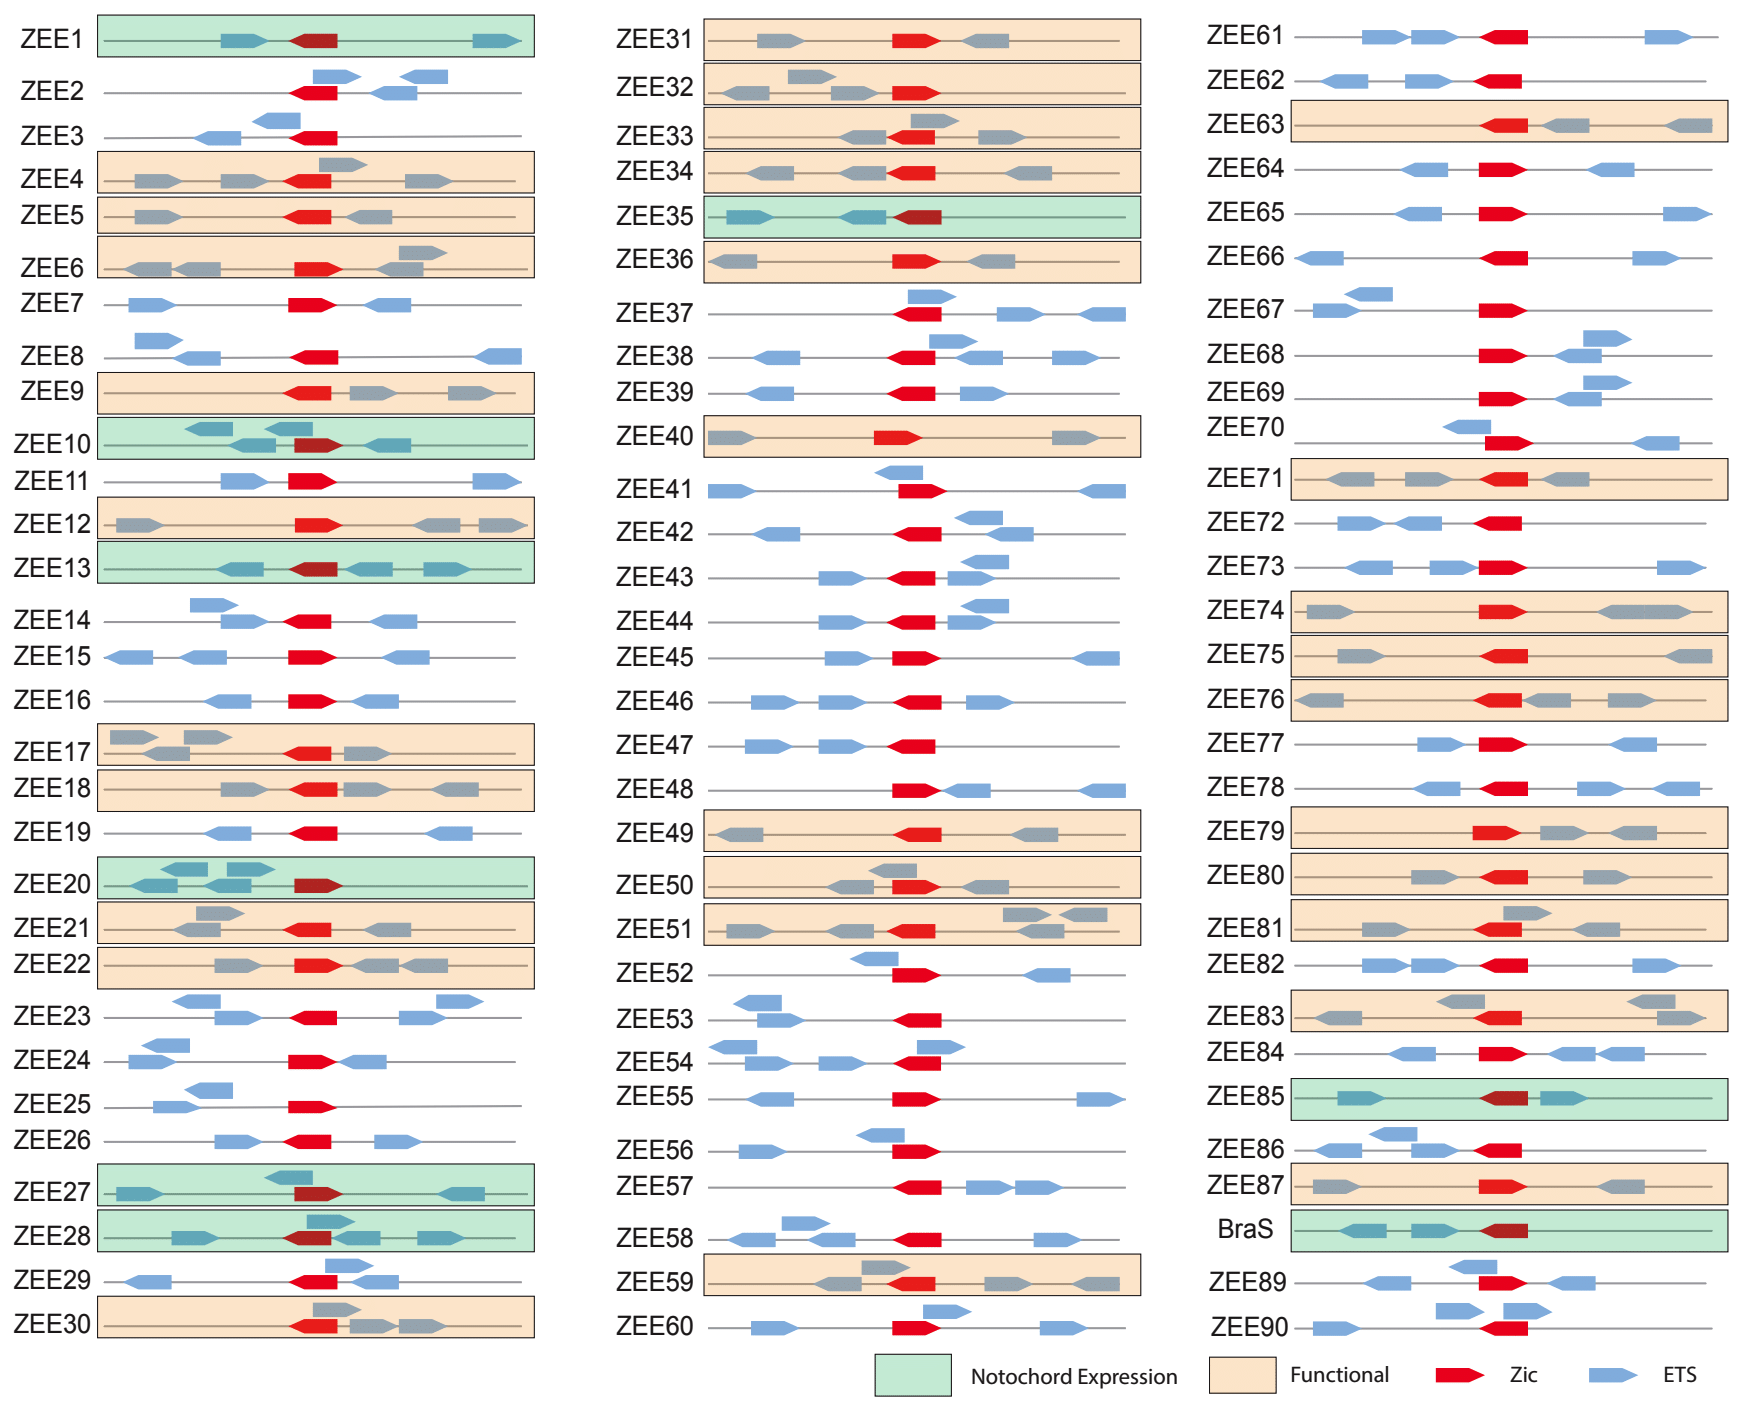
\includegraphics[scale=.2]{2_figures-and-files/FigS1_ZEE-Library.png}
    \caption[ZEE elements screened]{\textbf{ZEE elements screened.} Schematic of each ZEE element tested within our MPRA assay. Zic sites are colored red and ETS sites are colored blue. ZEE elements that were functional are boxed in orange. ZEE elements that drove notochord expression are boxed in green.}
    \label{fig:supplement zee elements screened}
\end{figure}

\begin{figure}[p]
    \centering
    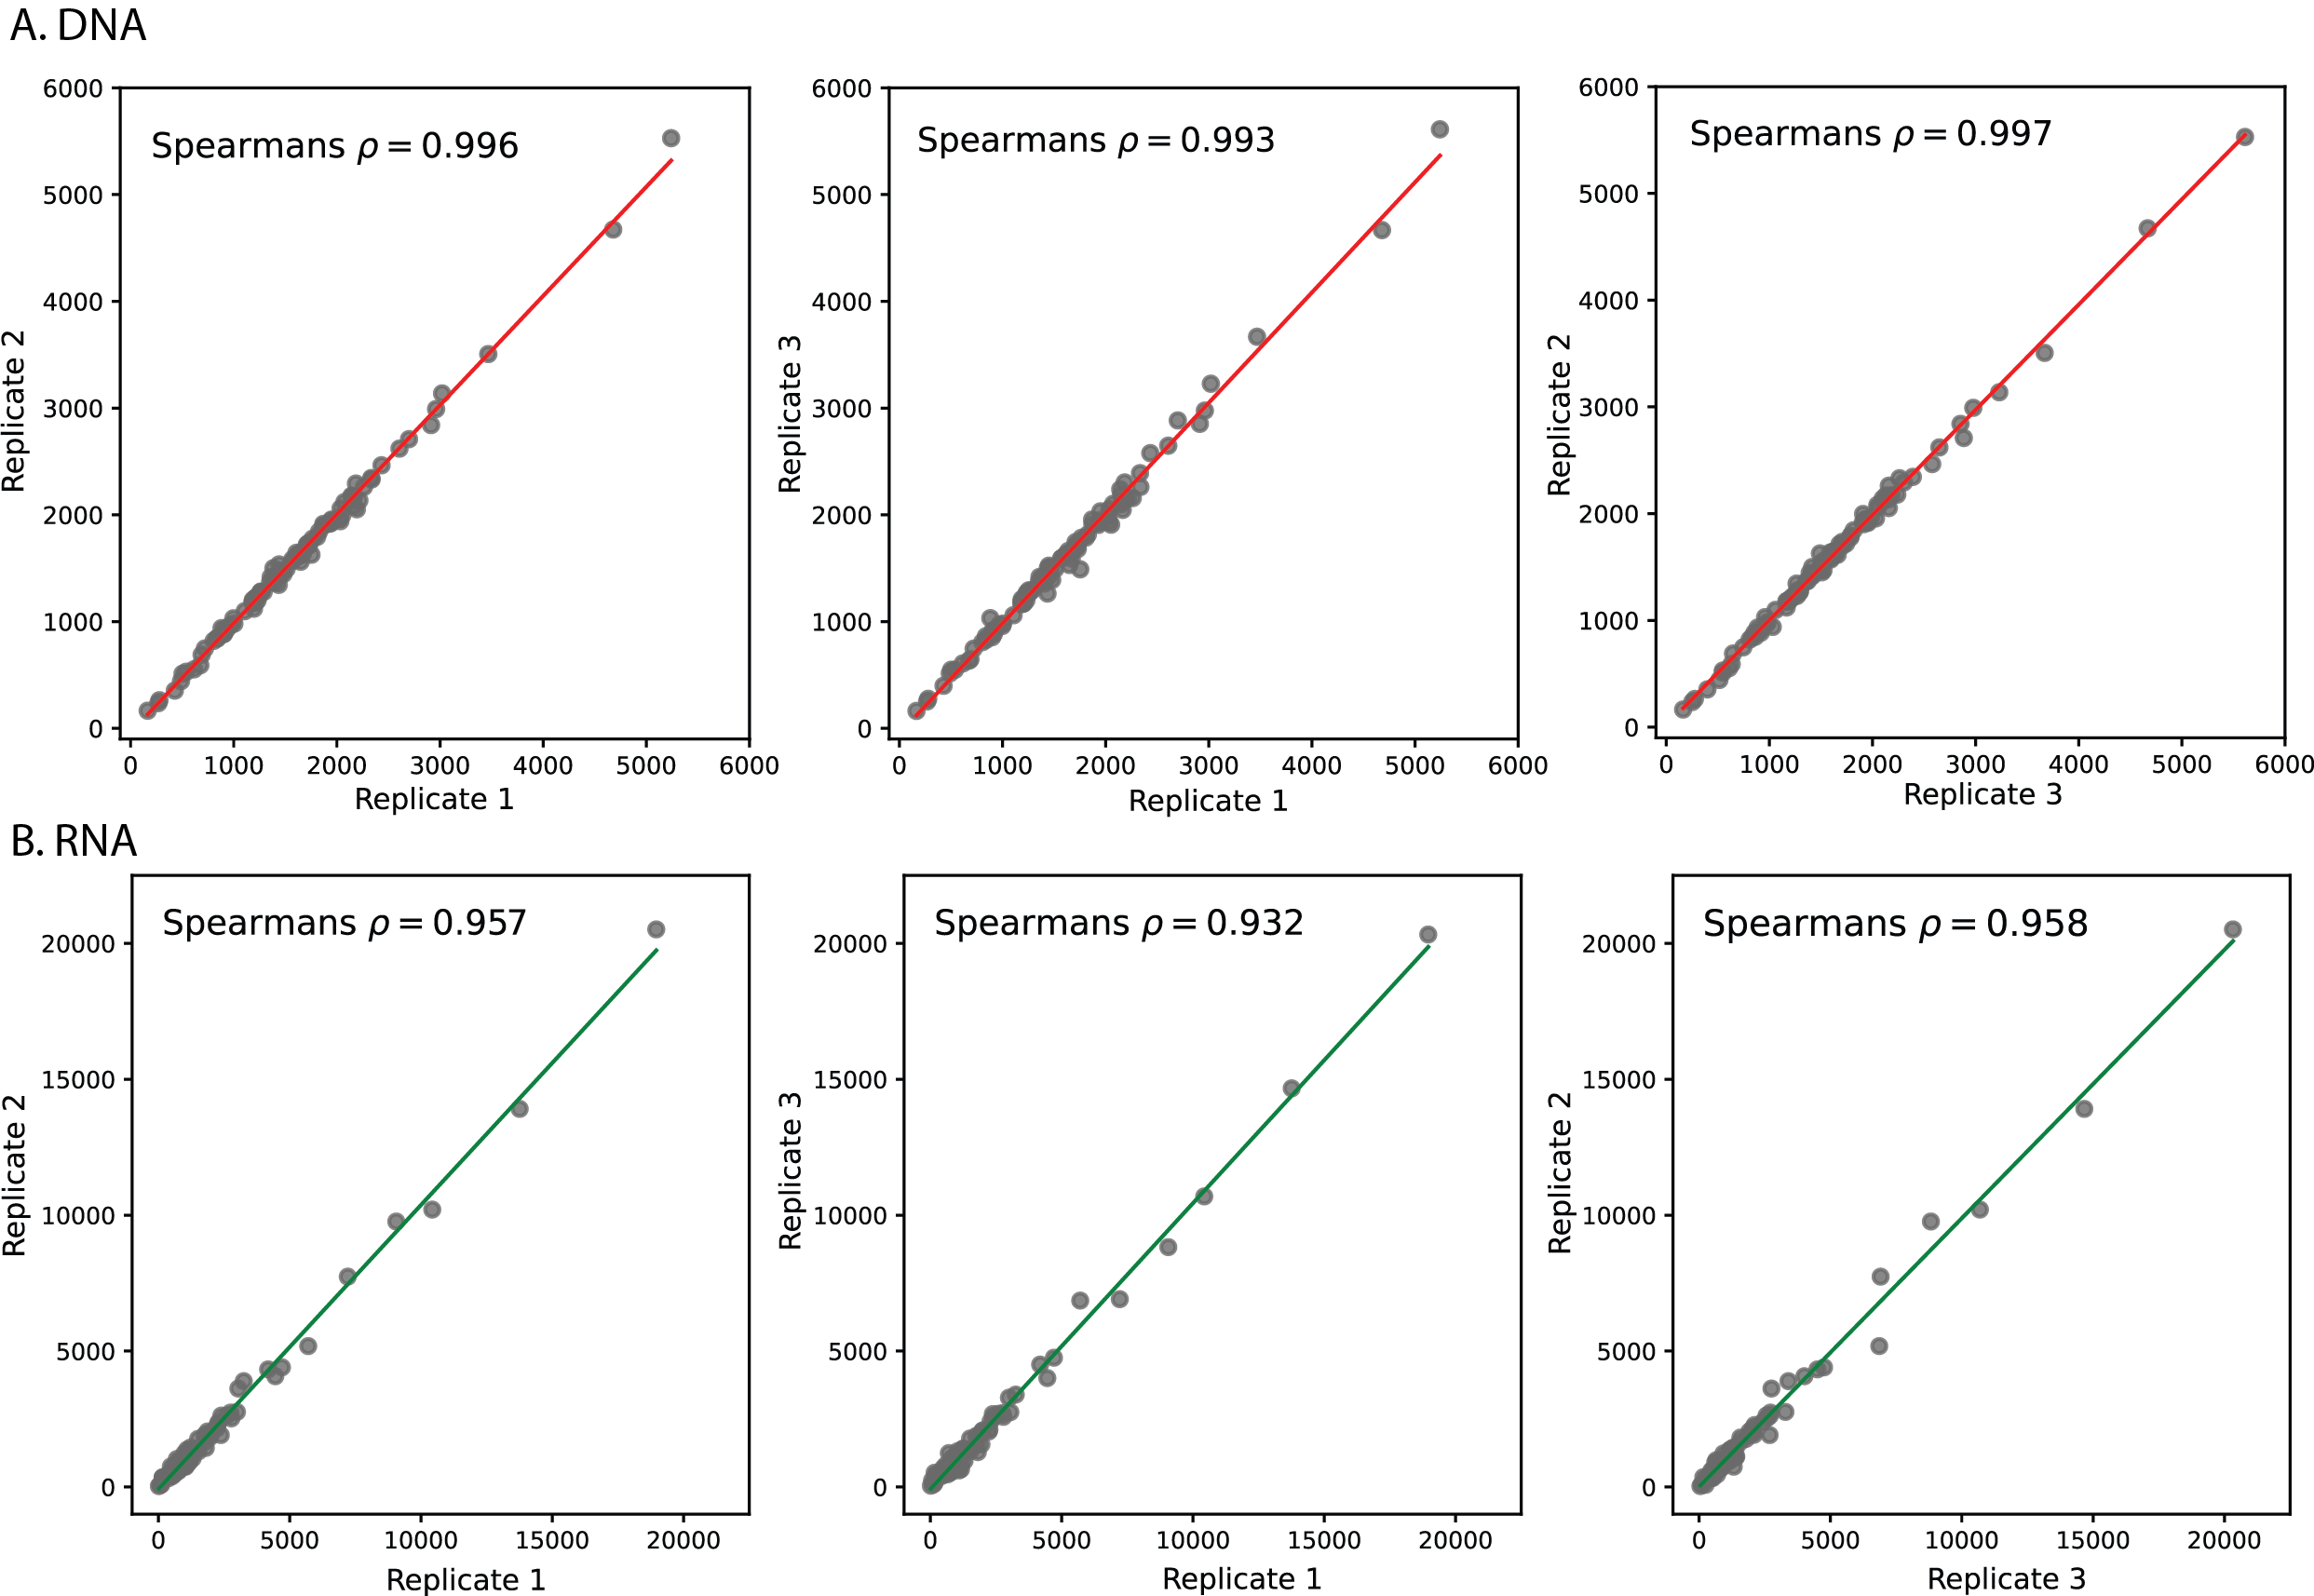
\includegraphics[scale=.75]{2_figures-and-files/FigS2_Data-QC.png}
    \caption[Data quality metrics illustrate high robustness of ZEE genomic screen]{\textbf{Data quality metrics illustrate high robustness of ZEE genomic screen.} \textbf{A.} Correlation of DNA plasmids detected between replicates was plotted. All Spearman correlations between replicates were $>$0.99. \textbf{B.} Correlation of mRNA barcodes detected between replicates was plotted. All Spearman correlations between replicates were $>$0.9.}
    \label{fig:supplement notochord data qc}
\end{figure}

\begin{figure}[p]
    \centering
    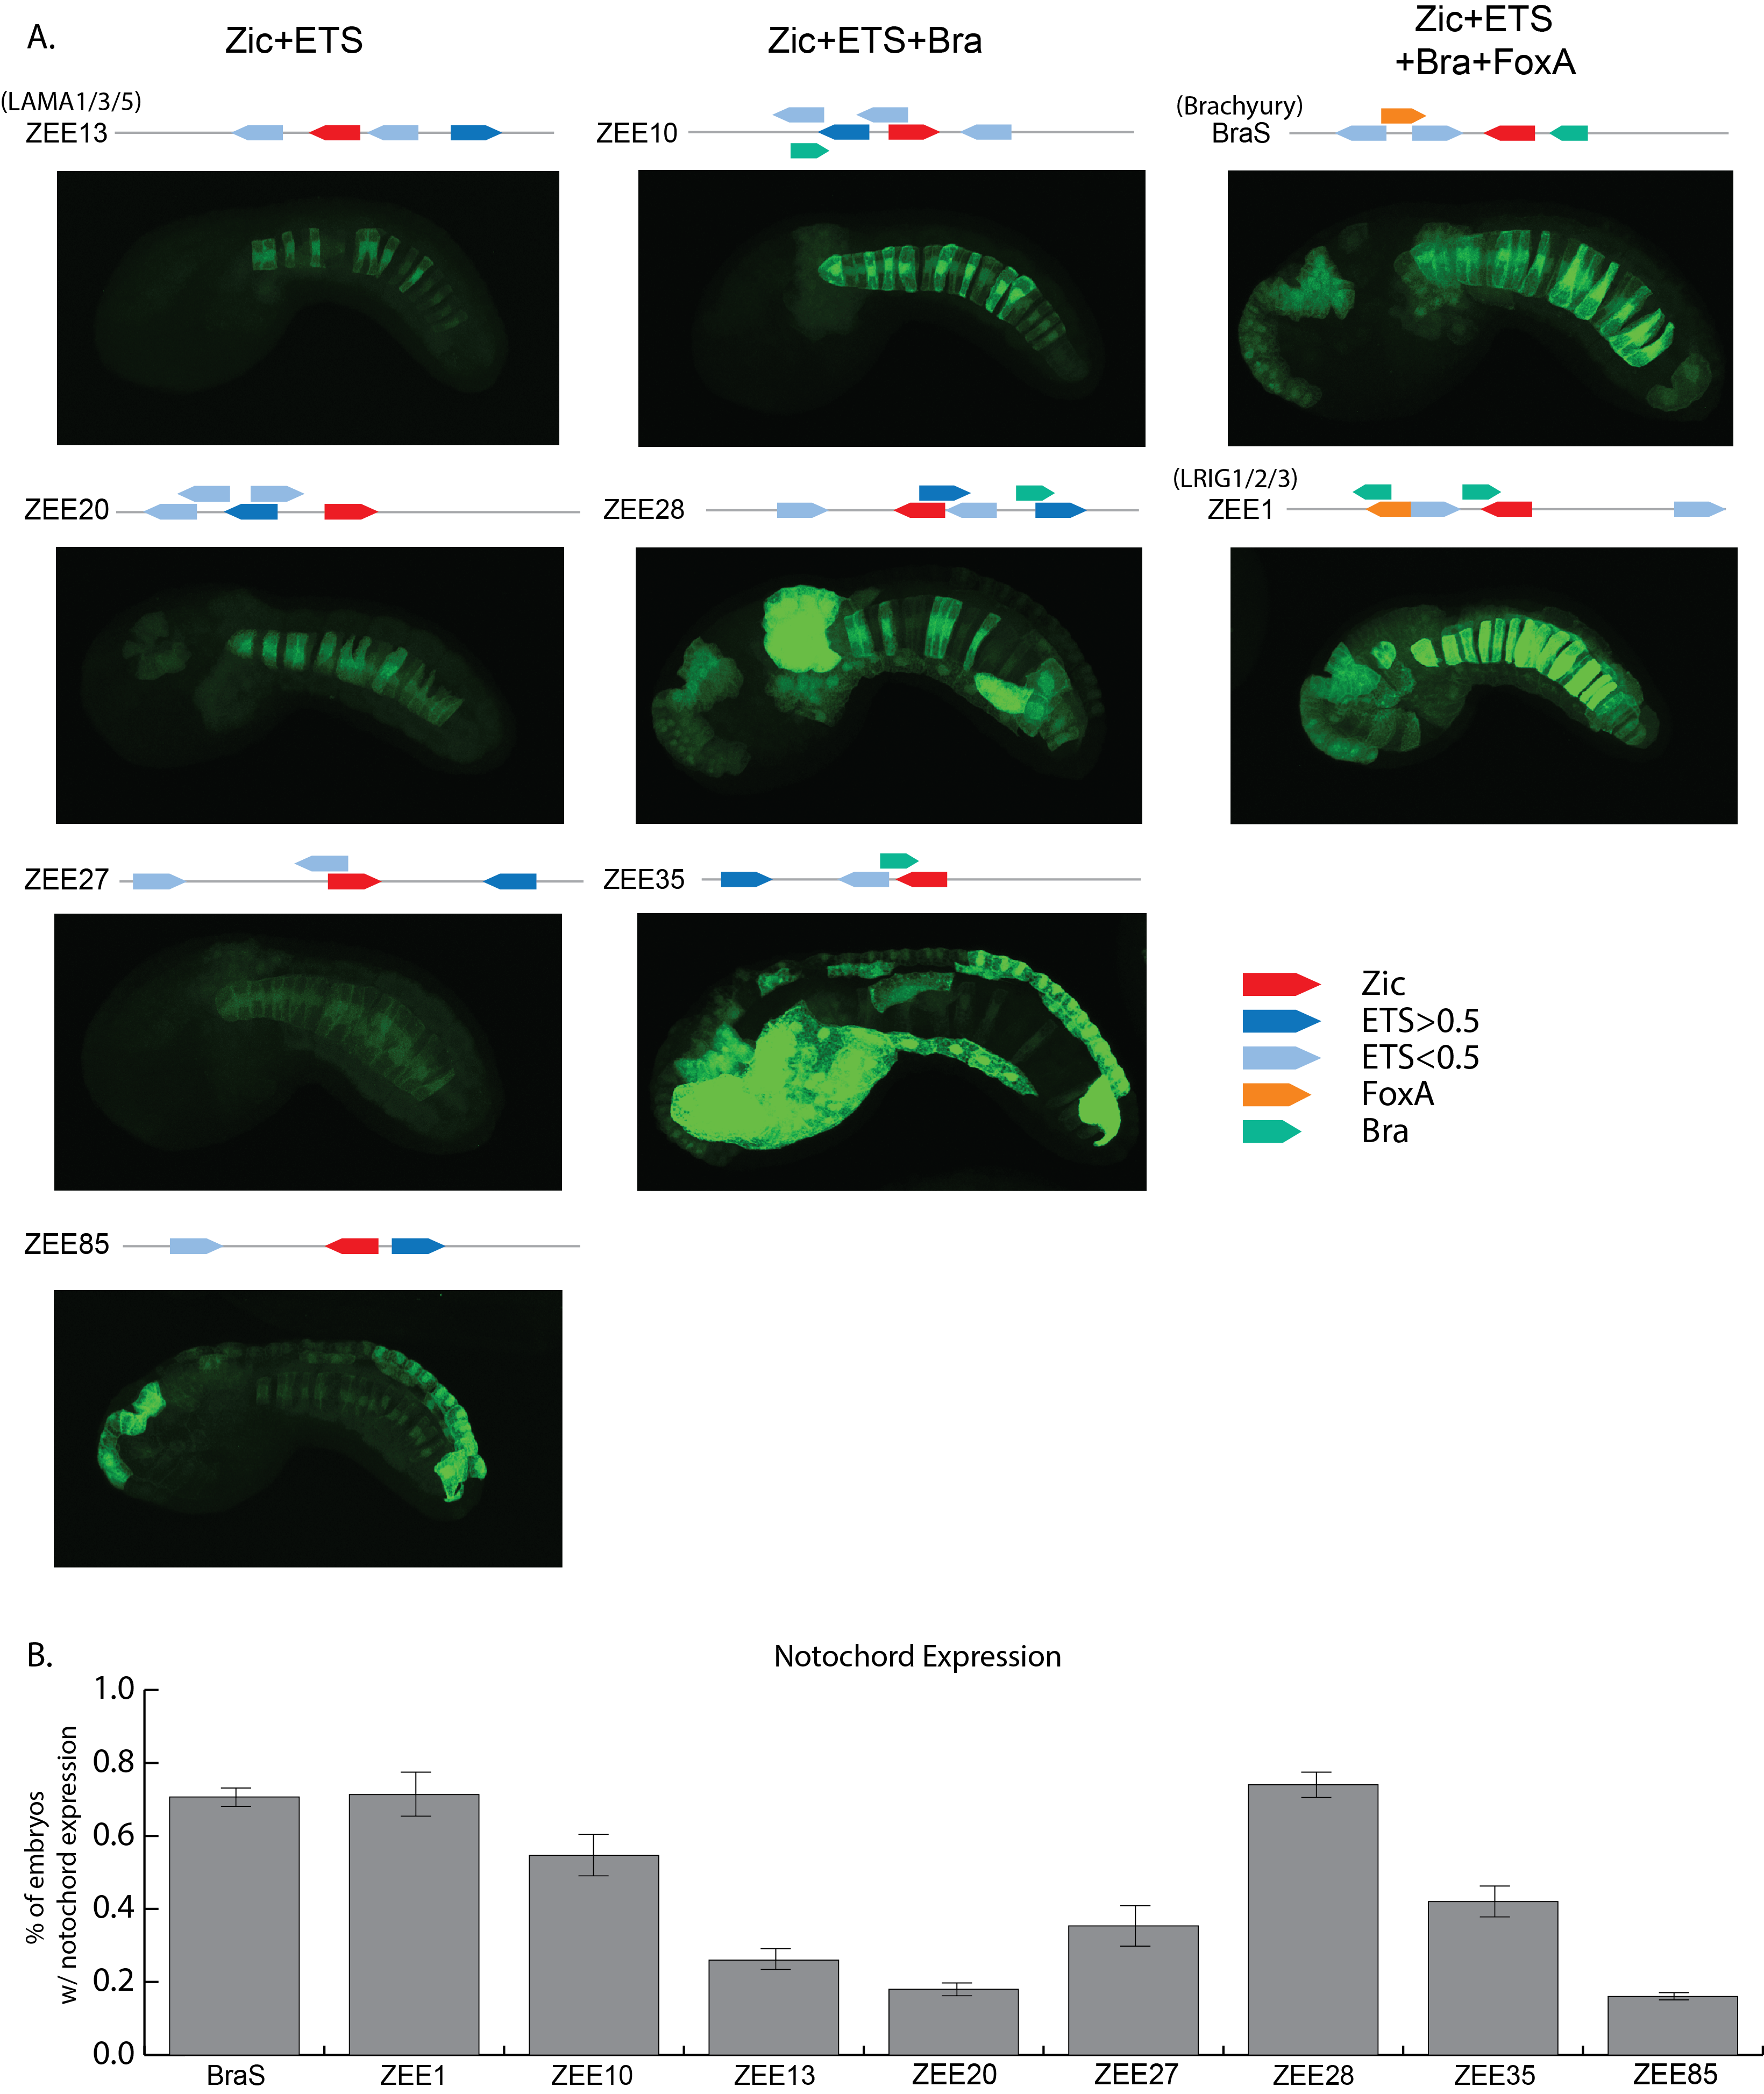
\includegraphics[scale=.55]{2_figures-and-files/FigS3_Notochord-Enhancers.png}
    \caption[Nine ZEE elements drive notochord expression]{\textbf{Nine ZEE elements drive notochord expression.} \textbf{A.} Images and schematics of the nine notochord enhancers in the ZEE library. Zic (red), ETS (blue), FoxA (orange), and Bra sites (green) are annotated. Dark blue ETS sites have an affinity of greater than 0.5, light blue sites have an affinity of less than 0.5. \textbf{B.} Counting data for nine ZEE elements showing the percentage of embryos with notochord expression. Three biological replicates were performed with 50 embryos per replicate analyzed.}
    \label{fig:supplement all notochord enhancers}
\end{figure}

\begin{figure}[p]
    \centering
    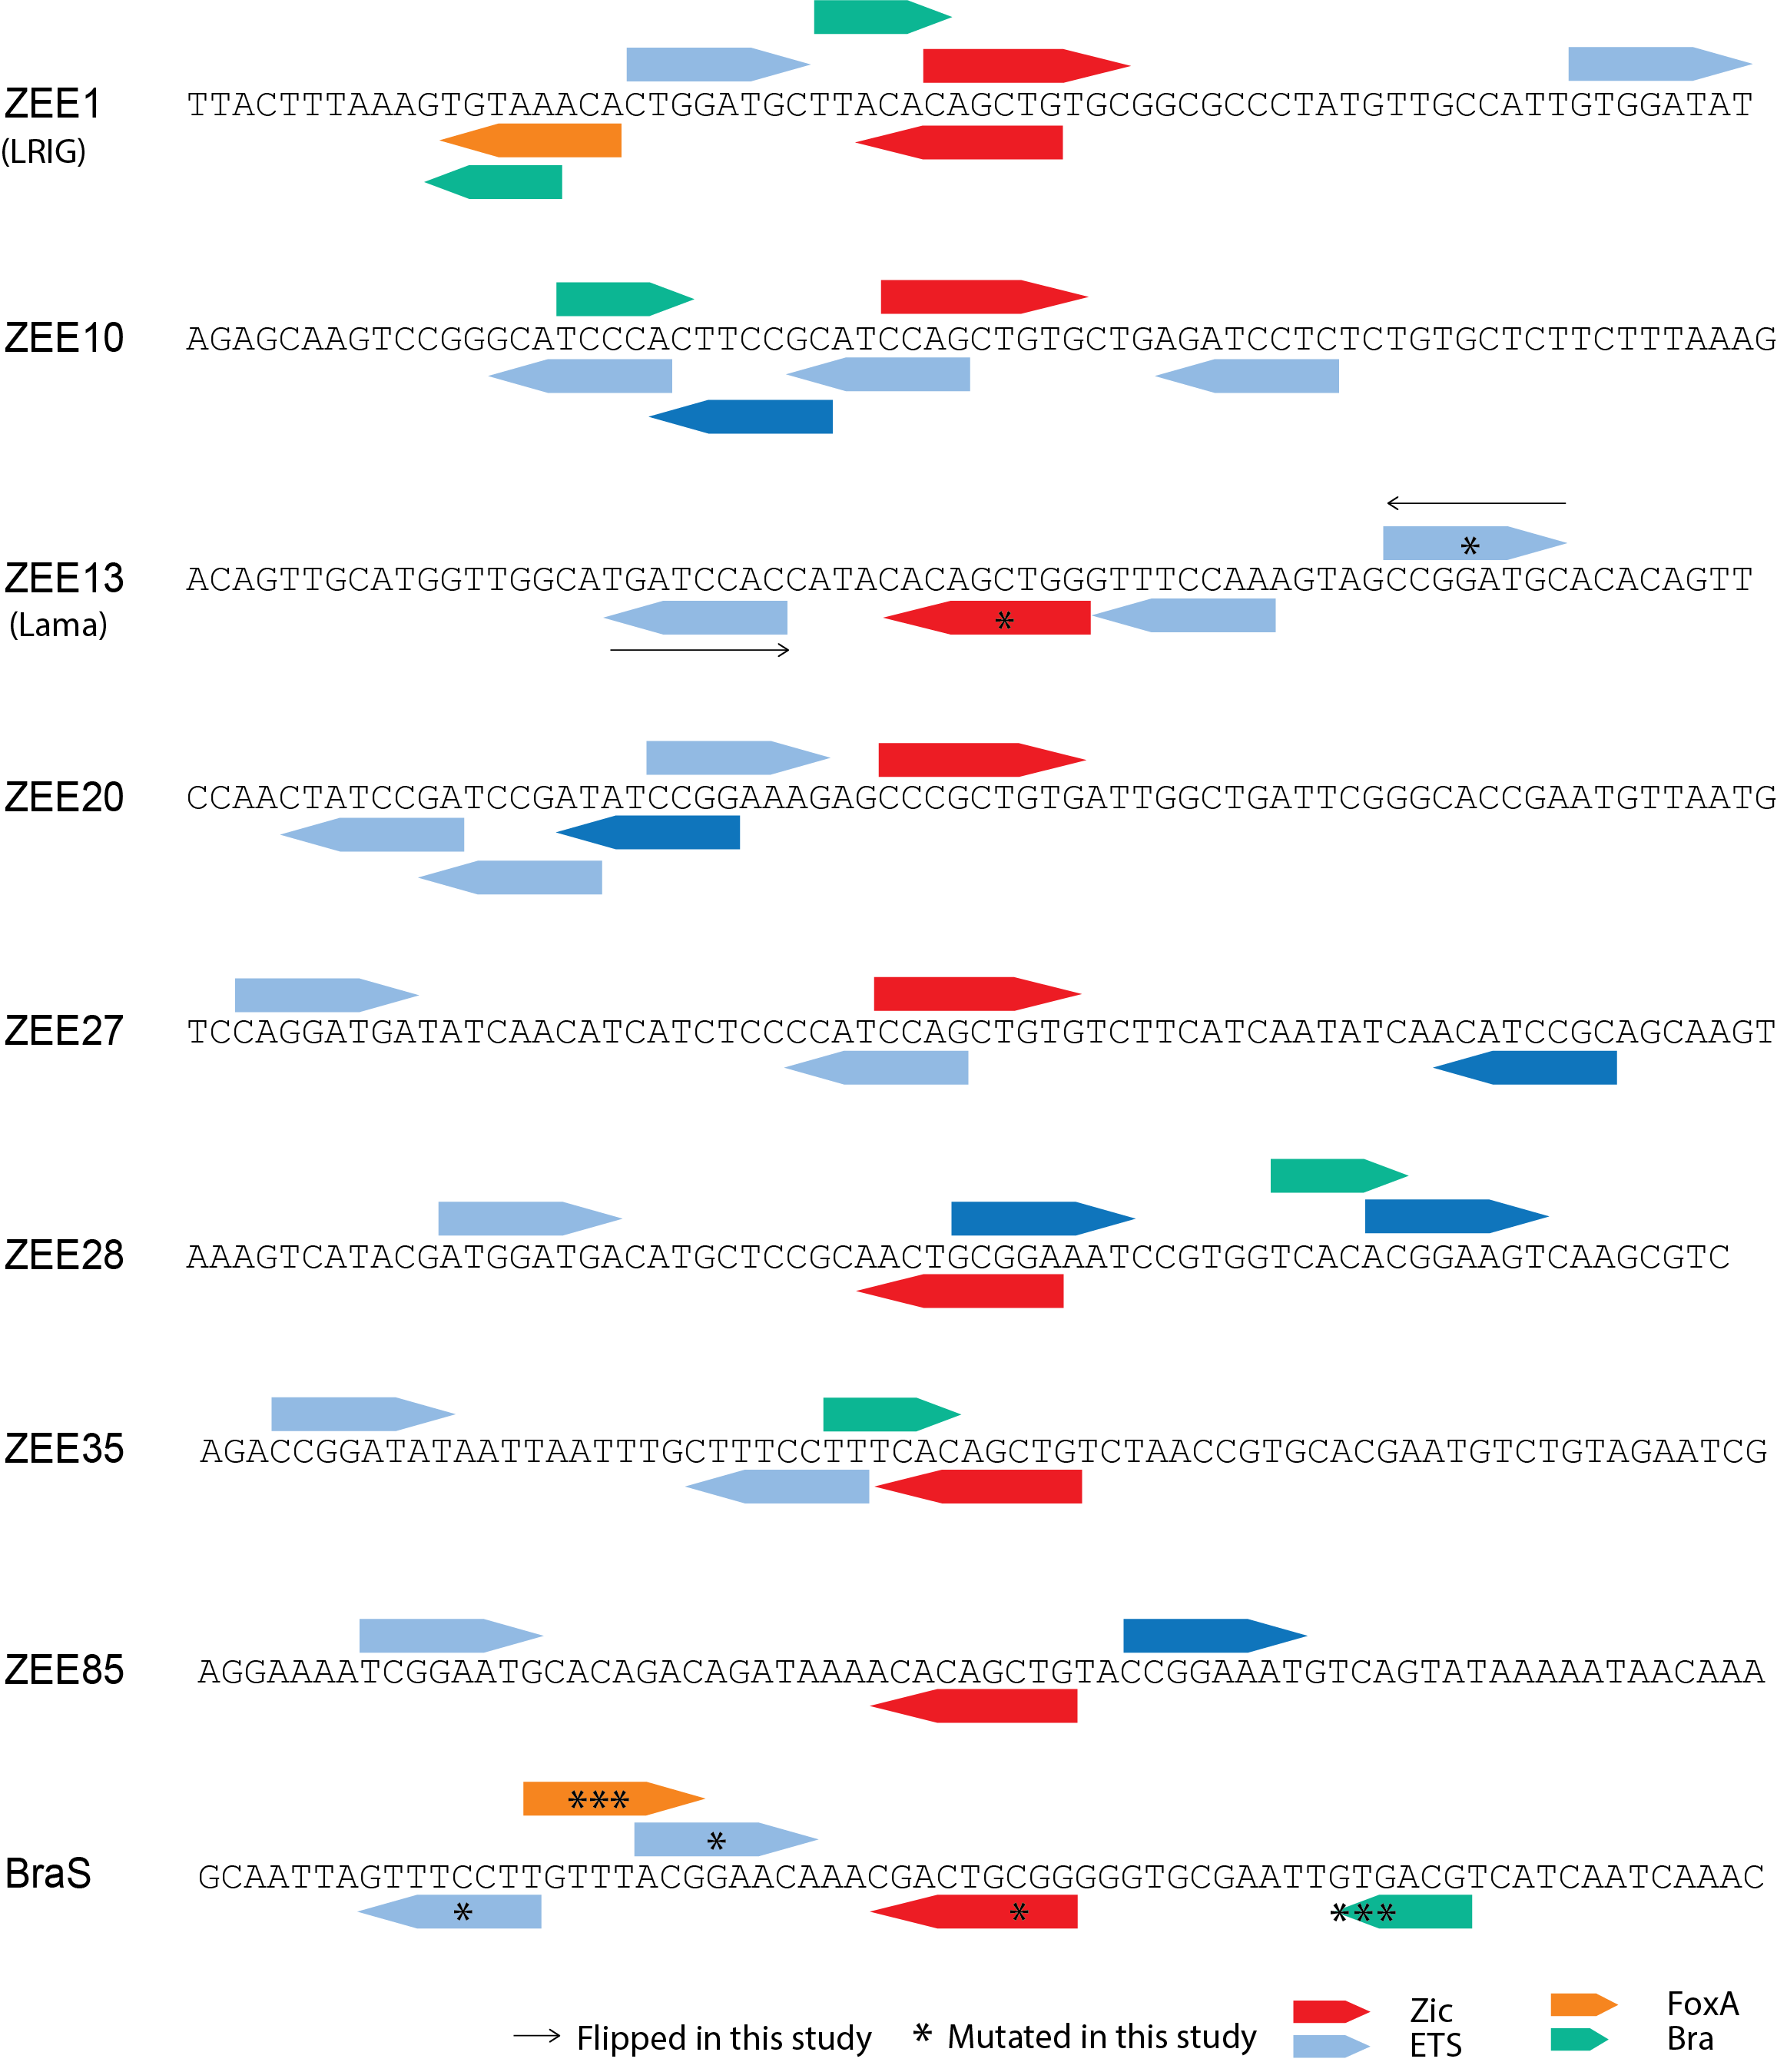
\includegraphics[scale=.75]{2_figures-and-files/FigS4_Notochord-Enhancer-Sequences.png}
    \caption[Annotated sequences of the nine ZEE elements that drive notochord expression]{\textbf{Annotated sequences of the nine ZEE elements that drive notochord expression.} Zic (red), ETS (blue), FoxA (orange), and Bra sites (green) are annotated. Asterisk denotes nucleotide that was mutated in this study, arrow denotes a binding site that was flipped. Dark blue ETS sites have an affinity of greater than 0.5, light blue sites have an affinity of less than 0.5.}
    \label{fig:supplement annotated zee elements}
\end{figure}

%%%%%%%%%%%% Figure S5 is large, so we need to split things! 
\begin{figure}[p]
    \centering
    \caption[Scoring of manipulated notochord enhancers]{\textbf{A.} Scoring of notochord expression for embryos electroporated with the \textit{laminin alpha} (Lama) enhancer, Lama -E3, Lama -Z, and Lama RE3. Lama -E3, Lama -Z, and Lama RE3 all show no notochord expression. \textbf{B.} Scoring of notochord expression for embryos electroporated with Bra Shadow (BraS), BraS -ZEE, BraS rZE, BraS -Bra, BraS –FoxA, and BraS rZEFB. BraS -ZEE, BraS rZE, BraS -Bra, and BraS –FoxA all show statistically significant less notochord expression compared to BraS, while BraS rZEFB is not significantly different. \textbf{C.} Scoring of levels of expression in the notochord for embryos electroporated with BraS and BraS rZEFB. BraS rZEFB shows less notochord expression levels compared to BraS. \textbf{D.} Scoring of a6.5 expression for embryos electroporated with BraS and BraS rZEFB. BraS rZEFB shows statistically significant less a6.5 expression compared to BraS. P values calculated by chi-squared test for expression levels and Fischer’s exact test for all other comparisons, * represents P$<$0.05, ** represents P$<$0.01. Dark blue ETS sites have an affinity of greater than 0.5, light blue sites have an affinity of less than 0.5. For counting data in Panel A, we conducted three biological repeats analyzing 50 embryos per replicate. For counting data shown in B, C, and D we conducted two biological repeats analyzing 50 embryos per replicate. (\textit{Continued on next page.})}
    \label{fig:supplement manipulated enhancers}
\end{figure}

\addtocounter{figure}{-1}

\captionsetup[figure]{list=no}
\begin{figure}[p]
    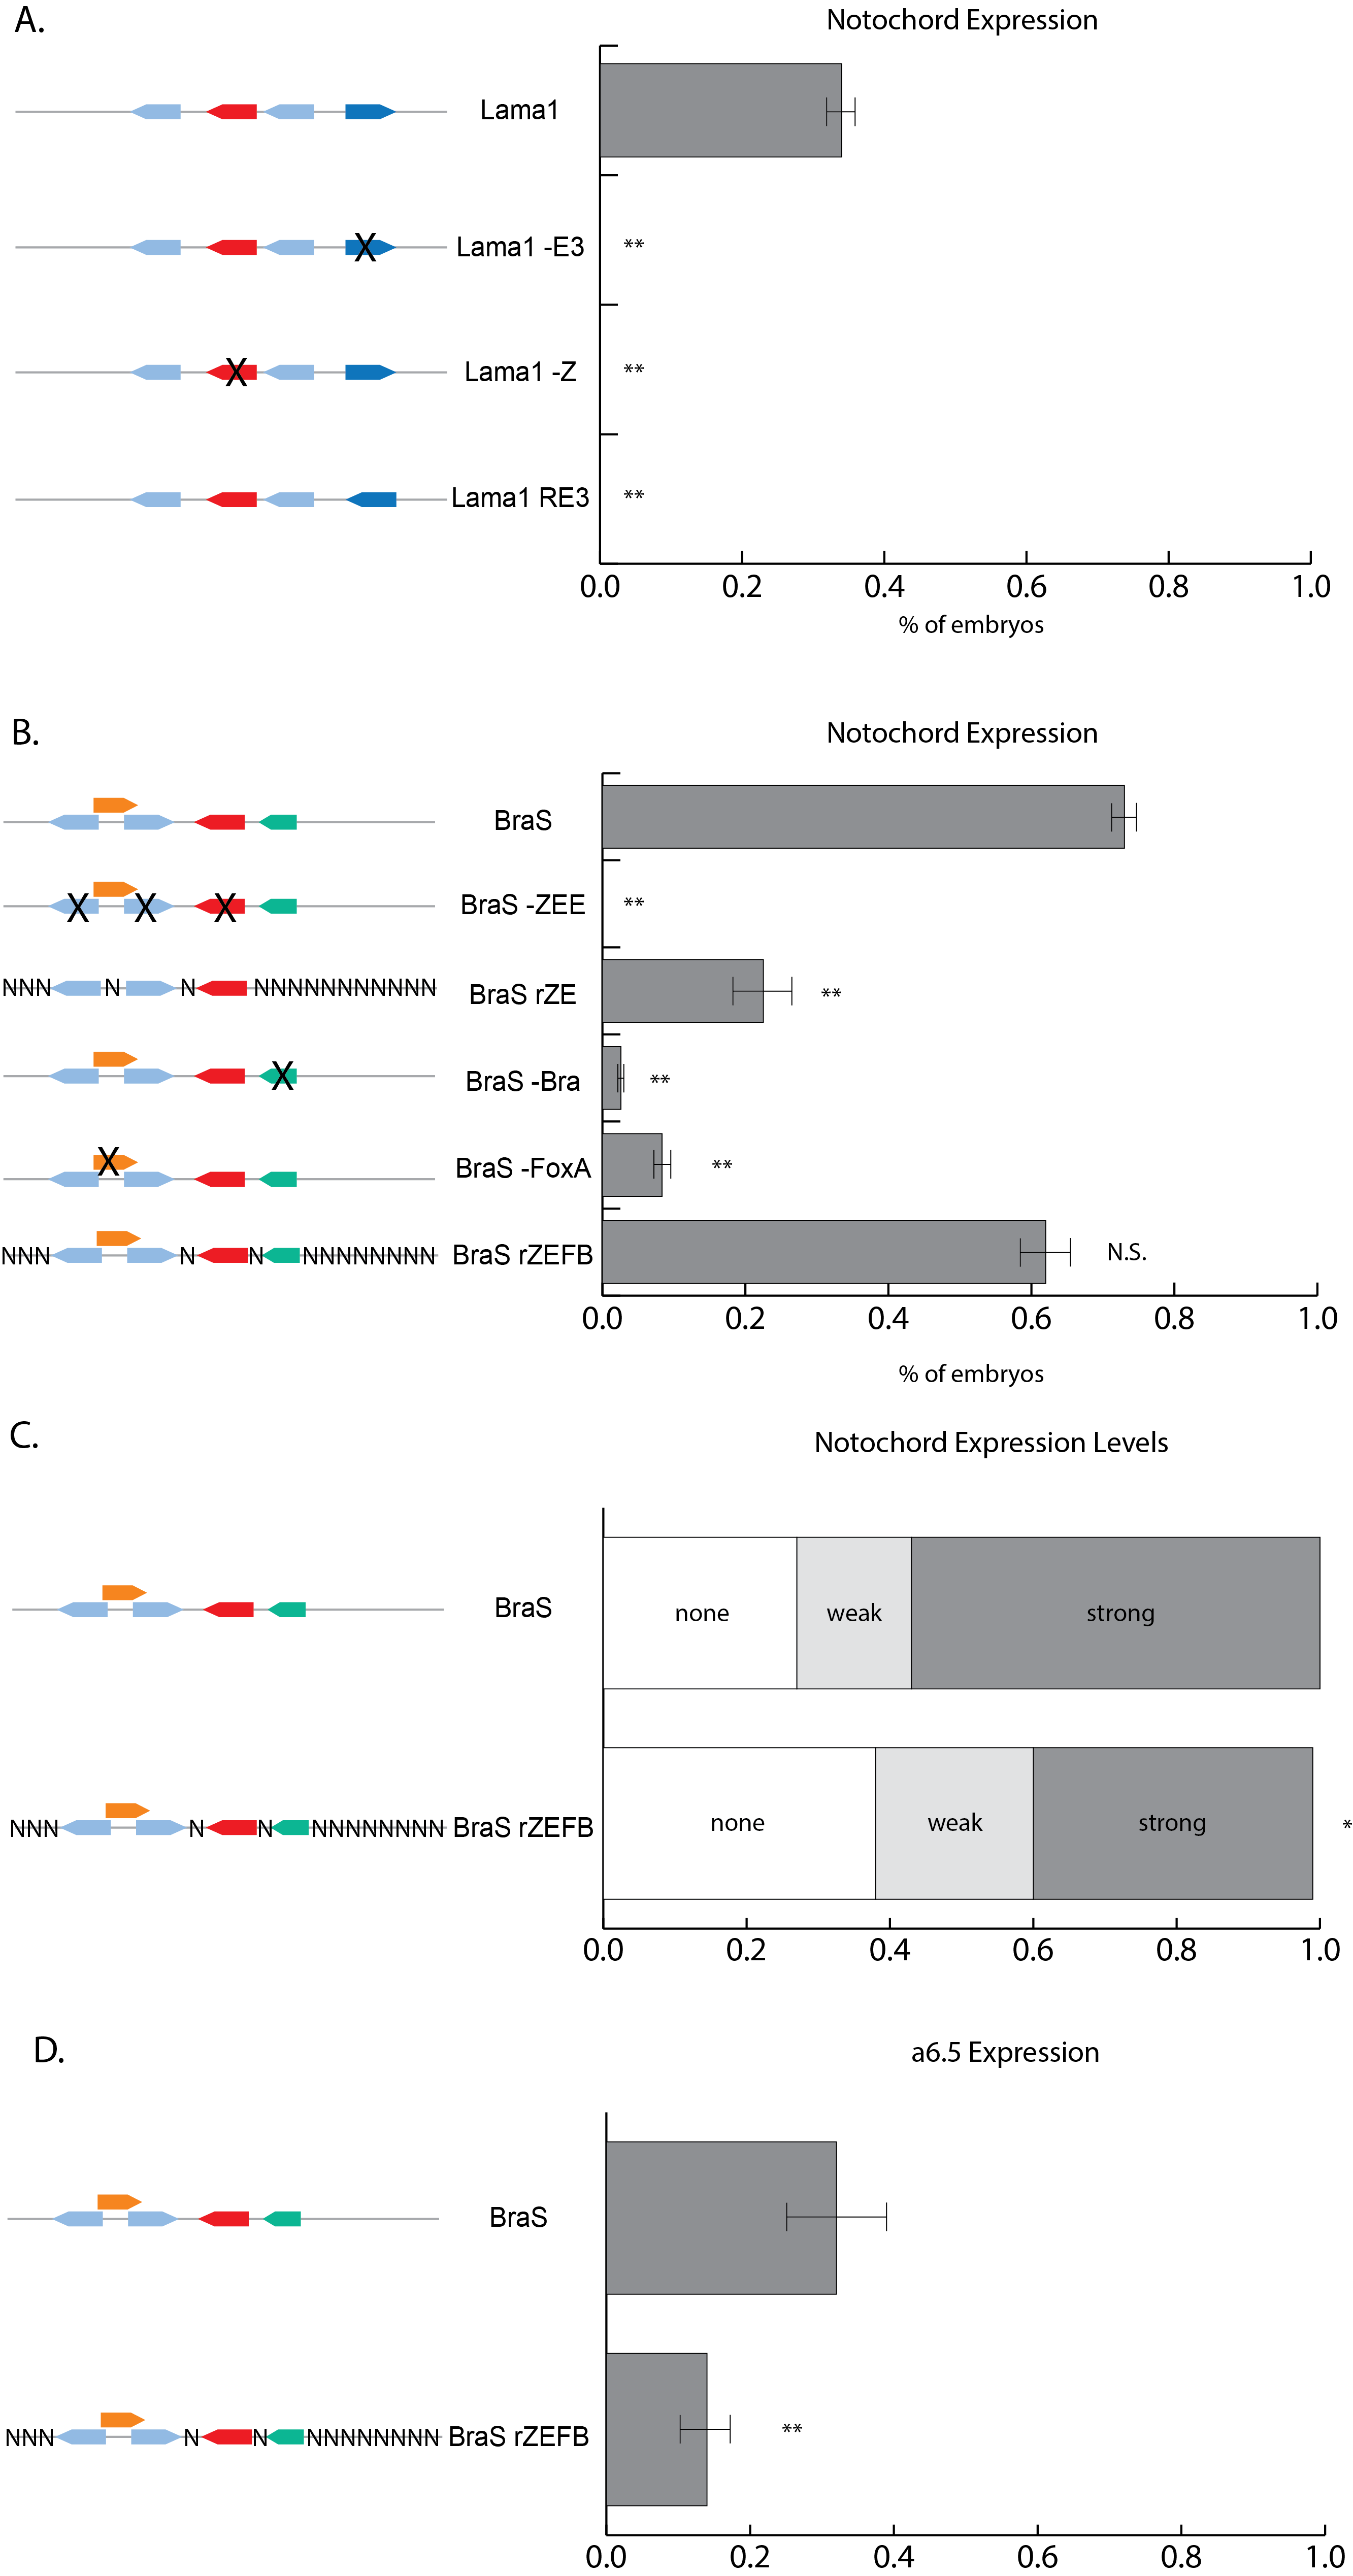
\includegraphics[scale=.5]{2_figures-and-files/FigS5_Notochord-Counting.png}
    \caption{(\textit{Continued from previous page.})}
\end{figure}
\captionsetup[figure]{list=yes}
%%%%%%%%%%%%

\begin{figure}[p]
    \centering
    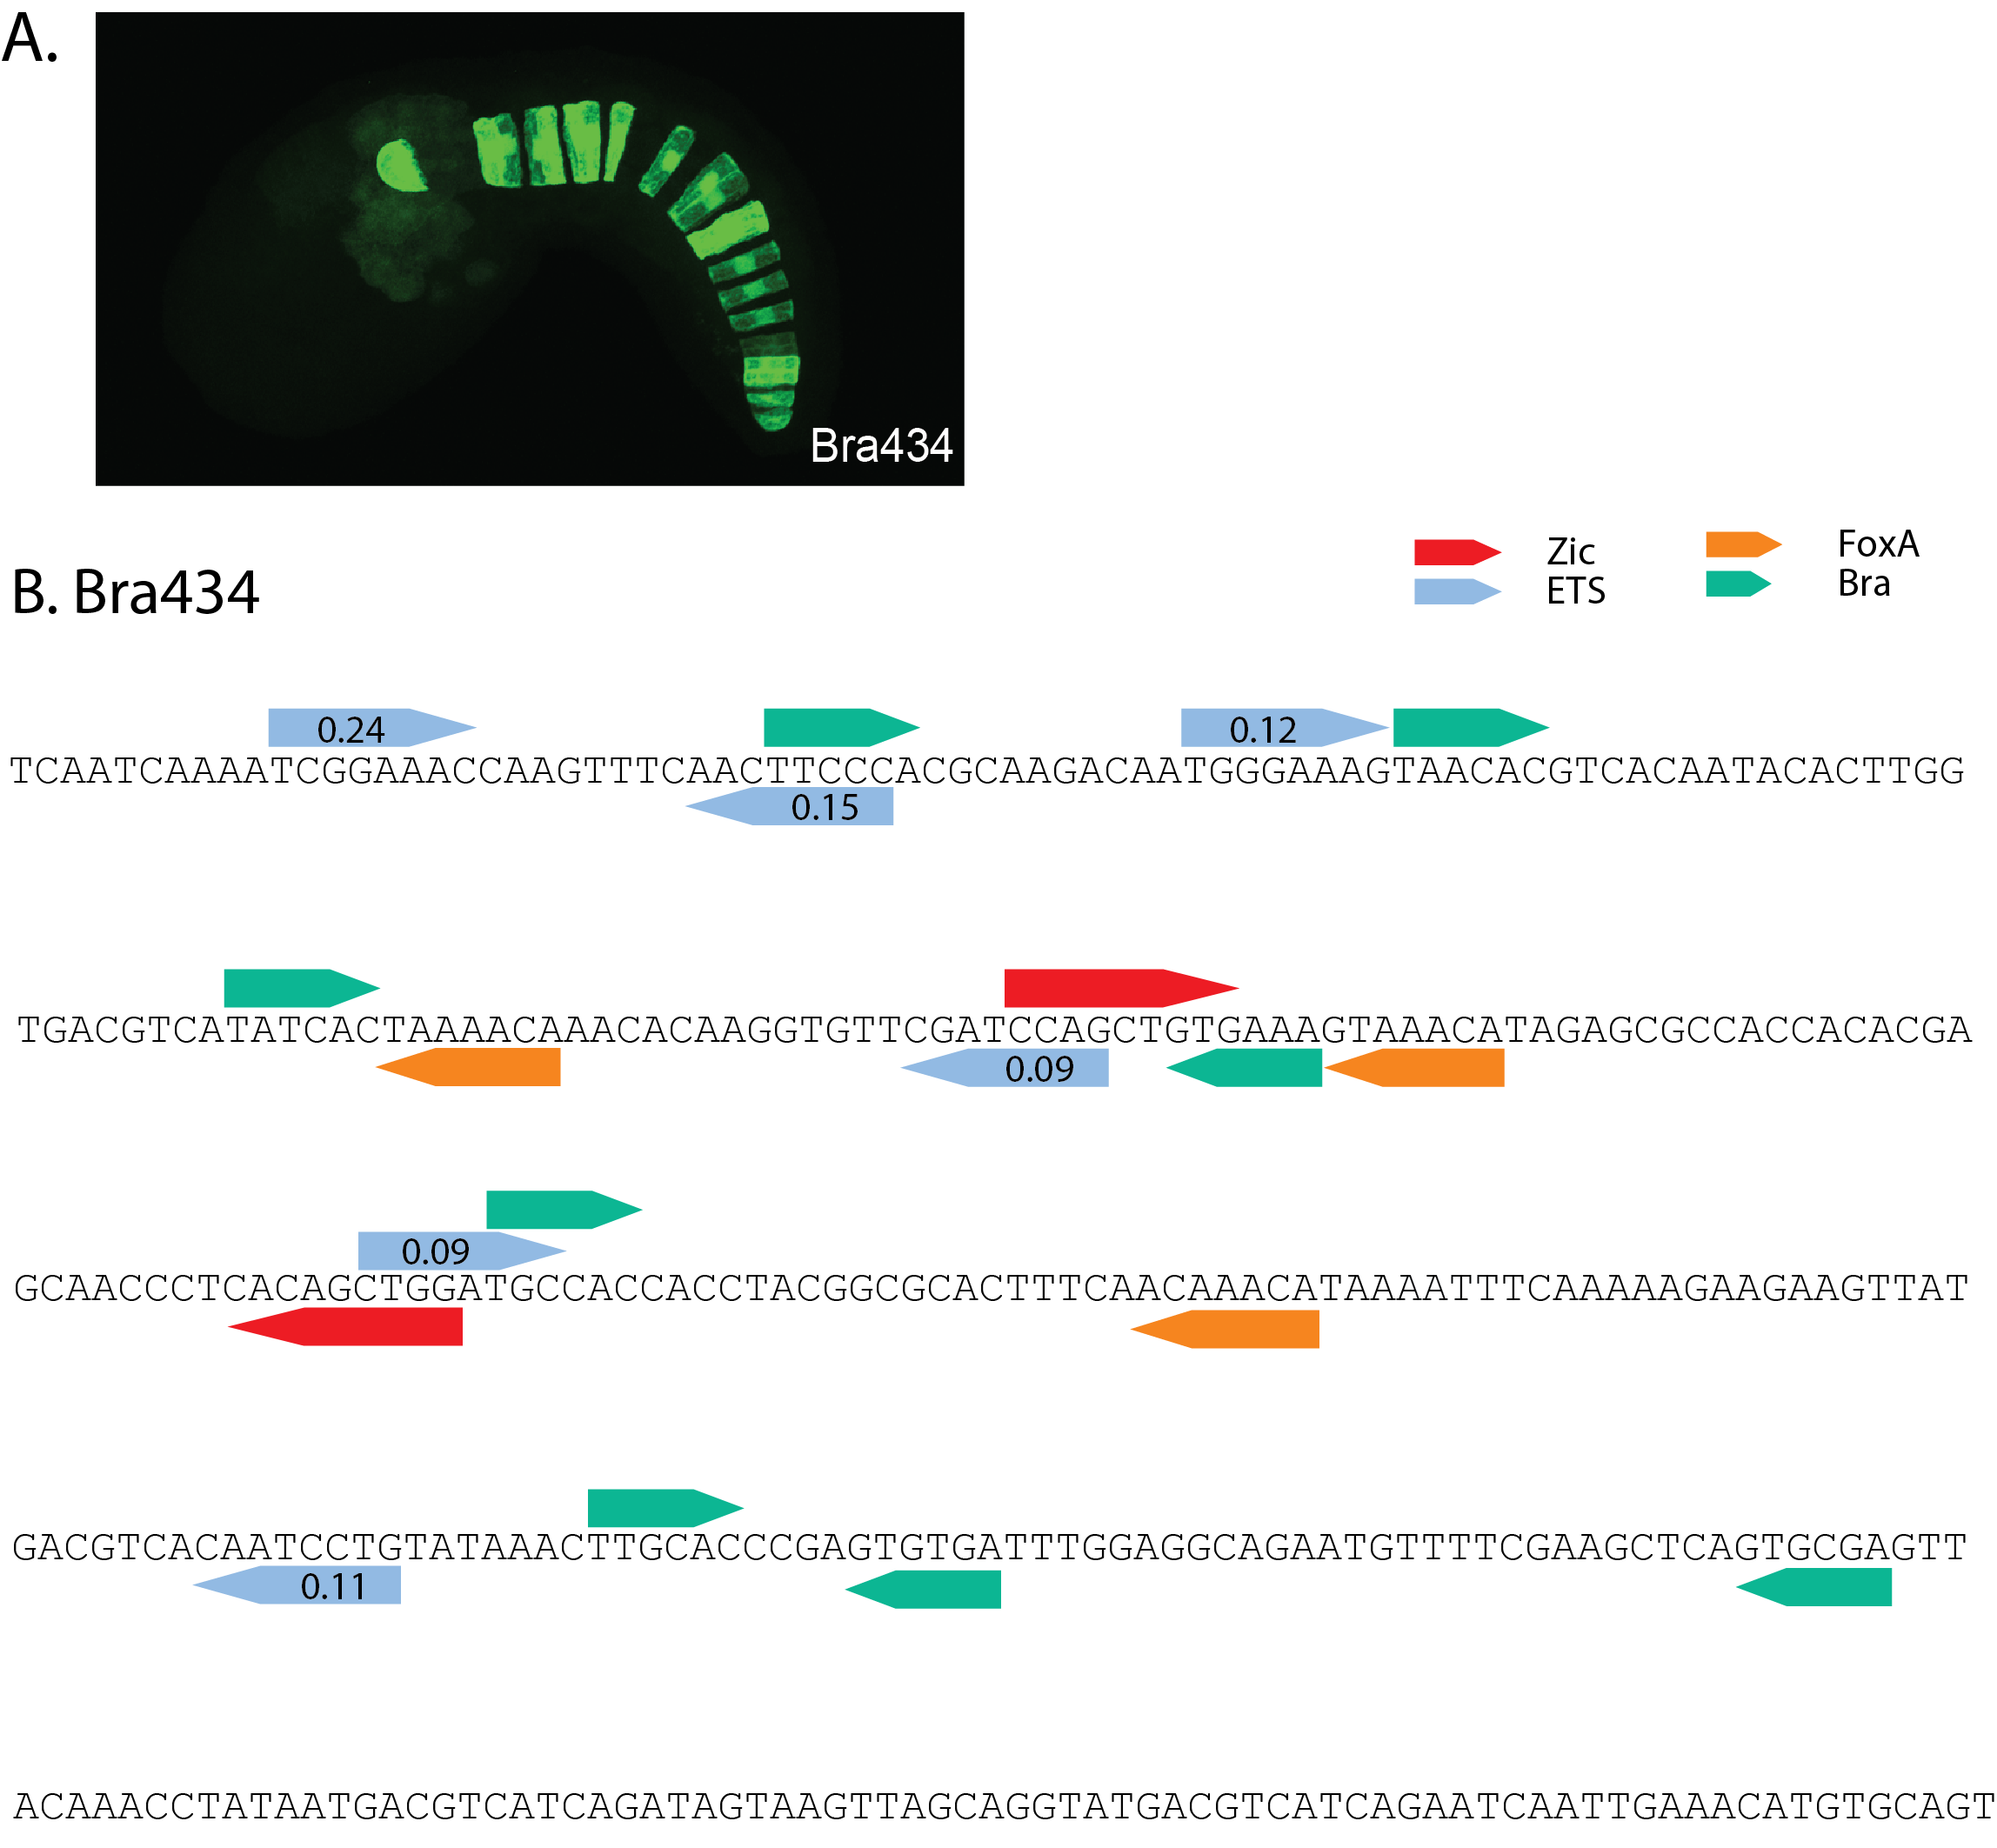
\includegraphics[scale=.65]{2_figures-and-files/FigS6_Bra434-Dissection.png}
    \caption[Updated annotation of Bra434]{\textbf{Updated annotation of Bra434.} \textbf{A.} Image of Bra434 electroporated into \textit{Ciona} embryo. \textbf{B.} Annotation of the Bra434 using PBM, EMSA, and crystal structure data . Zic sites in red, ETS sites in light blue, FoxA sites in orange, and Bra sites in green. Affinities of ETS calculated from PBM data (Wei et al., 2010) are labeled.}
    \label{fig:supplement bra434 annotated}
\end{figure}
